\chapter{Introduction}
\label{chp:intro}
\pagenumbering{arabic}


%%%%%%%%%%%%%%%%%%%%%%%%%%%%%%%%%%%%%%%%%%%%%%%%%%%%%%%%%%%%%%%%%%%%%%%%%%%%%%%%%%%%%%%%%%%%%%%%
\section{What Is \GrG?}

{\scshape GrGen} (\textsc{G}raph \textsc{R}ewrite \textsc{Gen}erator) is a software \emph{development tool} that offers \emph{programming languages} optimized for graph structured data, with declarative \emph{pattern matching} and \emph{rewriting} at their core, with support for imperative and object-oriented programming, and a bit of database-like query-result processing.
The generative programming system featuring a \emph{graphical debugger} eases the \emph{transformation} of \emph{graph-based representations}, as they are needed in e.g. engineering, model transformation, computer linguistics, or compiler construction.

%%%%%%%%%%%%%%%%%%%%%%%%%%%%%%%%%%%%%%%%%%%%%%%%%%%%%%%%%%%%%%%%%%%%%%%%%%%%%%%%%%%%%%%%%%%%%%%%
\section{When to Use \GrG}
You may be interested in using \GrG\ if you have to tackle the task of changing meshes of linked objects, i.e. \emph{graph-like data structures};
anytime the focus is on the \emph{relationship} in between your data entities,
and esp. if your algorithms operate upon data entities that stand in multiple relations to each other.

These tasks are traditionally handled by pointer structures and pointer structure navi\-gation-, search-, and replacement routines written by hand
-- this low-level, pointer-fiddling code can be generated automatically by \GrG\ for you.
You specify your transformation task on a \emph{higher level of abstraction} with nodes connected by edges,
and rewrite \emph{rules} consisting of \emph{patterns} to be searched as well as modifications to be carried out.
\GrG\ then generates the algorithmic core of your application.
You specify the \emph{what} with \emph{declarative rules}, \GrG\ takes care of the \emph{how};
similar to SQL expressions implemented by database engines, 
or to grammar rules implemented by parser generators.
Development is supported by \emph{visual debugging}, you work on a visualization of your network and the rule applications inside it.
The debugger and the pattern based languages boost your \emph{productivity} for graph-representation-based tasks way beyond traditional programming.
Due to all the optimizations implemented in the pattern matching engine you still gain \emph{high-performance} solutions.
Altogether, \GrG\ offers the highest combined speed of development and execution you can find for those kind of tasks.

%%%%%%%%%%%%%%%%%%%%%%%%%%%%%%%%%%%%%%%%%%%%%%%%%%%%%%%%%%%%%%%%%%%%%%%%%%%%%%%%%%%%%%%%%%%%%%%%
\section{An Example Graph-Based Representation}\label{sub:examplegraphrep}
Let's have a look at an example of a graph-based representation \GrG\ is well suited for 
-- a simplified version of the graph-based compiler intermediate representation \Firm\footnote{\url{www.libfirm.org}} that \textsc{GrGen} was originally developed for.
Nodes represent machine instructions, e.g.\ a \node{Load} fetches a value from an address or an \node{Add} sums two values.
Edges indicate dependencies between nodes, e.g.\ an \node{Add} requires that its two operands are available before it can be executed.
Each instruction is located within a basic block,
all nodes within the \node{Block} are executed if the \node{Block} is executed (in an order allowed by the dependencies).

\begin{figure}[htbp]
	\begin{minipage}[c]{0.43\textwidth}
		\centering
		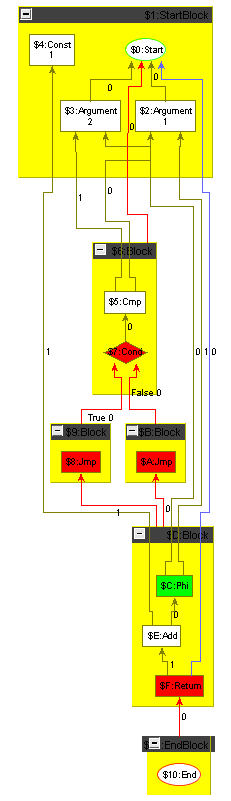
\includegraphics[width=2.3in]{fig/MinPlusNestedArguments.png}
	\end{minipage}
%
	\begin{minipage}[c]{0.57\textwidth}
		\centering
		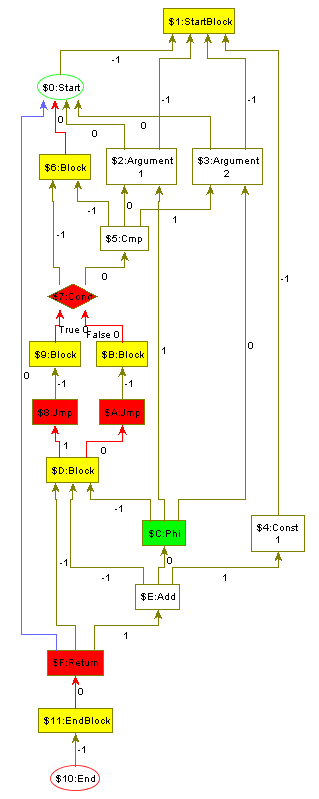
\includegraphics[width=3.3in]{fig/MinPlusPlainArguments.png}
	\end{minipage}
	\caption{Program graph of a minimum plus one function, with block containment visualized as containment left, and the plain graph right.}
	\label{fig:min}
\end{figure}

\autoref{fig:min} shows the program graph for the following C-function:

\pagebreak

\lstinputlisting{resources/MinPlus.c}

Program execution begins at the \node{Start} node, which also produces the initial memory state and the given \node{Argument}s.
The \node{Start} and the \node{Argument}s belong to the special \node{StartBlock}.
The \node{Cmp} compares the arguments, its result is used by the \node{Cond} to carry out a conditional jump depending on the result of the comparison.
After following the \node{Jmp} of the then- or the else-\node{Block}, the program execution is continued at \node{Block} \$D.
The \node{Phi}\footnote{a helper node from the static single assignment form employed; in \cite{braun13cc} you find more information and a simple algorithm for constructing SSA from an abstract syntax tree} 
chooses one of its operands depending on the previously executed block,
here \node{Argument} $1$ if the \node{Cond} was evaluated to \node{True},
or \node{Argument} $2$ if \node{Cond} was evaluated to \node{False}.
The \node{Const}ant 1 is added to the value selected by the \node{Phi},
before the result is returned by the \node{Return}.
The end of the program execution is represented by the special \node{EndBlock} which by convention contains exactly one \node{End}.
If you want to learn more about this representation or typical transformations over it, have a look at the compiler case\cite{CompilerCase} of the TTC 2011 where this representation was used or our solution \cite{CompilerOptimization}.

The key points here are that
\begin{enumerate}
	\item this is a mesh of objects (denoting operations),
	\item that stand to each other in 3 relations (control flow (red), data flow (brown), and memory flow (blue) \footnote{we use dependencies, i.e. the direction is reversed compared to the flow}), 
	\item and a major part of the information is encoded in the connection structure (topology),
	which is explicitly and directly represented with edges.
\end{enumerate}

You find such representations in other domains than \emph{programming languages} and \emph{compilers}, too.
The \emph{knowledge} of an agent about the exterior world can be \emph{represented} intuitively like this with \emph{semantic nets}, you could use \GrG\ for reasoning over them.
\emph{Models} as understood by \emph{model driven engineering} are typically graphs, with \GrG\ you can implement a model transformation between models, or into a lower-level program representation.
When working in \emph{computational linguistics} you may be interested in modeling an \emph{abstract syntax graph} in \GrG;
the recursive and iterated patterns that allow to process tree-like data structures declaratively render \GrG\ an excellent match for such tasks.
But also in \emph{engineering} or \emph{architecture} where you need to describe the buildup of the modeled system from components, here you can derive context-sensitively system \emph{blueprints} or simulate their behaviour.
You find help not only in modelling them, but also in deriving all interesting configurations or simulating all interesting execution traces. 
In form of the built-in support for a backtracking search through a search space or even the enumeration of a state space with isomorphic state pruning, guided by match ordering and filtering.


%%%%%%%%%%%%%%%%%%%%%%%%%%%%%%%%%%%%%%%%%%%%%%%%%%%%%%%%%%%%%%%%%%%%%%%%%%%%%%%%%%%%%%%%%%%%%%%%
\section{When Not to Use \GrG}
There is nothing to gain from \GrG\ if scalars, lists or arrays are sufficient to model your domain,
which is the case for a lot of tasks in computing indeed.
(But which is not the case for others which would be better modeled with trees and especially graphs,
but aren't because of the cost of maintaining pointer structures by hand.)
\GrG\ is likely too heavyweight if you are just interested in computing shortest paths in simple graphs.
You're better off with a traditional graph library and its set of pre-implemented algorithms --
the library can be learned quicker and the algorithms can be reused directly.
\GrG\ with its domain-specific languages in contrast requires time to learn and some effort to specify or code a solution in (only afterwards are you rewarded with a much higher pace of development).

The graph rewrite generator is not the right tool for you if you're searching for a visual environment to teach children programming -- it's a powerful tool for (software) engineers.
Simpler and less powerful languages like story diagrams\cite{storydiagrams} that can be learned quicker and understood more intuitively may be a better match here.
Neither is it what you need if your graph structured data is to be interactively edited by an end user instead of being automatically transformed by rules (the editor generator DiaGen\cite{diagen} may be of interest in this case).

Each object-oriented program contains a heap of objects pointing to each other that can be understood as a graph like representation, with objects being the nodes and the references being the (fixed) edges.
In contrast to object-oriented programming is the topology in graph-oriented programming as offered by \GrG\ not hidden and encapsulated in the objects, but globally open for inspection and modification;
open and readily accessible for pattern matching and rewriting.
Prefer the closed heaps if you don't need a global view on the data, they are cheaper and the information hiding cuts dependencies.

%If you don't need to map one complete representation to another complete representation,
%or if you don't need to match and rewrite patterns inside a representation,
%you are likely better off with the stronger information hiding of object-oriented programming.
%-- it leads to a better software system architecture.
%A certain level of information hiding is offered with hierarchical graphs as offered by \GrG, though.
%The graph inside an attribute is shielded from the graph containing it.


%%%%%%%%%%%%%%%%%%%%%%%%%%%%%%%%%%%%%%%%%%%%%%%%%%%%%%%%%%%%%%%%%%%%%%%%%%%%%%%%%%%%%%%%%%%%%%%%
\section{What Is Graph Rewriting?}\indexmain{graph rewriting}
\label{ov:whatsallabout}

The notion of graph rewriting as understood by \GrG\ is a method for declaratively specifying ``changes'' to a graph.
This is comparable to the well-known term rewriting.
Normally you use one or more \newterm{graph rewrite rules} to accomplish a certain task.
\GrG\ implements an SPO-based approach (as default).
In the simplest case such a graph rewrite rule consists of a tuple $L \rightarrow R$, whereas $L$---the \newterm{left hand side}\indexmainsee{LHS}{left hand side} of the rule---is called \newterm{pattern graph} and $R$---the \newterm{right hand side}\indexmainsee{RHS}{right hand side} of the rule---is the \newterm{rewrite graph}.

\begin{figure}[htbp]
	\centering
  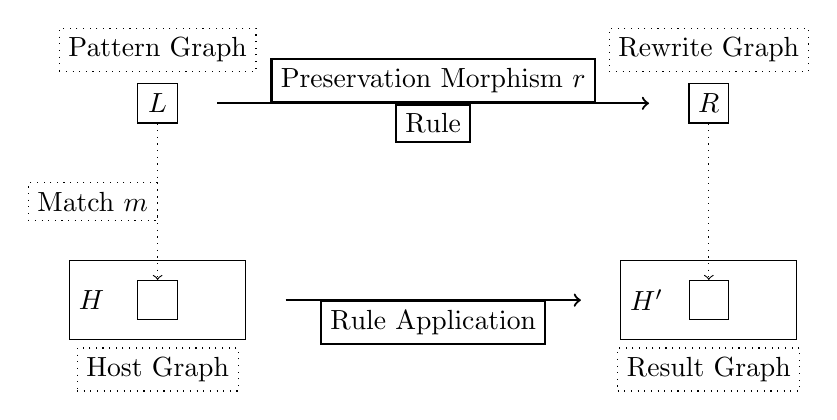
\begin{tikzpicture}
    \begin{scope}[minimum size=0.5cm]
      \tikzstyle{every node}=[draw]
      \node (L)     at (0   ,2.5) {$L$};
      \node (R)     at (7   ,2.5) {$R$};
      \node (mL)    at (0   ,0) {};
      \node (mR)    at (7   ,0) {};
      \node[text width=2cm,text badly ragged,minimum size=1cm] (H)     at (0   ,0) {$H$};
      \node[text width=2cm,text badly ragged,minimum size=1cm] (Hs)    at (7   ,0) {$H'$};
    \end{scope}

    \draw[dotted,->] (L) node[above=0.4cm] {Pattern Graph} -> (mL) node[left,midway]  {Match $m$}   node[below=0.6cm] {Host Graph};
    \draw[dotted,->] (R) node[above=0.4cm] {Rewrite Graph} -> (mR)                              node[below=0.6cm] {Result Graph};

    \pgfsetshortenstart{0.5cm}
    \pgfsetshortenend{0.5cm}
    \draw[thick,->]  (L) -> (R)  node[above,midway] {Preservation Morphism $r$} node[below,midway] {Rule};
    \draw[thick,->]  (H) -> (Hs) node[below,midway] {Rule Application};
  \end{tikzpicture}
  \caption{Basic Idea of Graph Rewriting}
  \label{figrule}
\end{figure}

Moreover we need to identify graph elements (nodes or edges) of $L$ and $R$ for preserving them during rewrite.
This is done by a \newterm{preservation morphism} $r$ mapping elements from $L$ to $R$; the morphism $r$ is injective, but needs to be neither surjective nor total.
Together with a rule name $p$ we have $p : L \xrightarrow{r} R$.

The transformation is done by \newterm{application}\indexmainsee{rule application}{application} of a rule to a \newterm{host graph} $H$.
To do so, we have to find an occurrence of the pattern graph in the host graph.
Mathematically speaking, such a \newterm{match} $m$ is an isomorphism from $L$ to a subgraph of $H$.
This morphism may not be unique, i.e.\ there may be several matches.
Afterwards we change the matched \indexed{spot} $m(L)$ of the host graph, such that it becomes an isomorphic subgraph of the rewrite graph $R$.
Elements of $L$ not mapped by $r$ are deleted from $m(L)$ during rewrite.
Elements of $R$ not in the image of $r$ are inserted into $H$, all others (elements that are mapped by $r$) are retained.
The outcome of these steps is the resulting graph $H'$. In symbolic language: $H \xRightarrow{m, p} H'$.


%%%%%%%%%%%%%%%%%%%%%%%%%%%%%%%%%%%%%%%%%%%%%%%%%%%%%%%%%%%%%%%%%%%%%%%%%%%%%%%%%%%%%%%%%%%%%%%%
\section{An Example For Rewriting}\indexmain{example}
\label{ov:example}

We'll have a look at a small example.
Graph elements (nodes and edges) are labeled with an identifier.
If a type is necessary then it is stated after a colon.
We start using a special case to construct our host graph: an \indexed{empty pattern} always produces exactly one\footnote{Because of the uniqueness of the total and totally undefined morphism.} match (independent of the host graph). So we construct an apple by applying
\[
  p_0:
  \begin{array}[c]{c}
    \emptyset
  \end{array}
  \begin{array}[c]{c}
    \longrightarrow
  \end{array}
  \begin{array}[c]{c}
    \begin{tikzpicture}[show background rectangle]
      \tikzstyle{every node}=[circle]
      \node[draw] (n1) at (2.5,5) {};
      \node[draw] (n2) at (2,4)   {};
      \node[draw] (n3) at (0,2)   {};
      \node[draw] (n4) at (2,0)   {};
      \node[draw] (n5) at (4,2)   {};

    	\draw[-latex] (n2) --                                  (n1) node[left,midway]  {$e_1$};
    	\draw[-latex] (n2) .. controls +(-1,1) and +(0,1) ..   (n3) node[left,midway]  {$e_2$};
      \draw[-latex] (n3) .. controls +(0,-1) and +(-1,0) ..  (n4) node[left,midway]  {$e_3$};
    	\draw[-latex] (n4) .. controls +(1,0)  and +(0,-1) ..  (n5) node[right,midway] {$e_4$};
      \draw[-latex] (n5) .. controls +(0,1)  and +(1,1) ..   (n2) node[right,midway] {$e_5$};
    \end{tikzpicture}
  \end{array}
\]
to the empty host graph.
As the result we get an apple as new host graph $H$.
Now we want to rewrite our apple with stem to an apple with a leaflet.
So we apply
\[
  p_1:
  \begin{array}[c]{c}
    \begin{tikzpicture}[show background rectangle]
      \tikzstyle{every node}=[circle,minimum size=0.7cm]
      \node[draw] (a) at (2,5.5)  {a};
      \node[draw] (b) at (2,4)    {b};

    	\draw[-latex] (b) -- (a) node[left,midway]  {$x$};
    \end{tikzpicture}
  \end{array}
  \begin{array}[c]{c}
    \longrightarrow
  \end{array}
  \begin{array}[c]{c}
    \begin{tikzpicture}[show background rectangle]
      \tikzstyle{every node}=[circle,minimum size=0.7cm]
      \node[draw] (c) at (2,5.5)  {c};
      \node[draw] (b) at (2,4)    {b};

    	\draw[-latex] (b) .. controls +(-0.7,+0.7) and +(-0.7,-0.7) .. (c) node[left,midway]   {$y$};
    	\draw[-latex] (b) .. controls +(+0.7,+0.7) and +(+0.7,-0.7) .. (c) node[right,midway]  {$z$};
    \end{tikzpicture}
  \end{array}
\]
to $H$ and get the new host graph $H_1$, something like this:
\[
  \begin{array}[c]{c}
    \begin{tikzpicture}[show background rectangle]
      \tikzstyle{every node}=[circle]
      \node[draw] (n1) at (2.5,5) {};
      \node[draw] (n2) at (2,4)   {};
      \node[draw] (n3) at (0,2)   {};
      \node[draw] (n4) at (2,0)   {};
      \node[draw] (n5) at (4,2)   {};

    	\draw[-latex] (n2) --                                  (n1) node[left,midway]  {$e_1$};
    	\draw[-latex] (n2) .. controls +(-1,1) and +(0,1) ..   (n3) node[left,midway]  {$e_2$};
      \draw[-latex] (n3) .. controls +(0,-1) and +(-1,0) ..  (n4) node[left,midway]  {$e_3$};
    	\draw[-latex] (n4) .. controls +(1,0)  and +(0,-1) ..  (n5) node[right,midway] {$e_4$};
      \draw[-latex] (n5) .. controls +(0,1)  and +(1,1) ..   (n2) node[right,midway] {$e_5$};
    \end{tikzpicture}
  \end{array}
  \begin{array}[c]{c}
    \xRightarrow{\quad p_1 \quad}
  \end{array}
  \begin{array}[c]{c}
    \begin{tikzpicture}[show background rectangle]
      \tikzstyle{every node}=[circle]
      \node[draw] (n1) at (2.5,5) {};
      \node[draw] (n2) at (2,4)   {};
      \node[draw] (n3) at (0,2)   {};
      \node[draw] (n4) at (2,0)   {};
      \node[draw] (n5) at (4,2)   {};
      \node[draw] (n6) at (0,0.5)   {};

    	\draw[-latex] (n2) --                                  (n1) node[left,midway]  {$e_1$};
    	\draw[-latex] (n2) .. controls +(-1,1) and +(0,1) ..   (n3) node[left,midway]  {$e_2$};
      \draw[-latex] (n3) .. controls +(-0.7,-0.7) and +(-0.7,+0.7) .. (n6) node[left,midway]  {$e_6$};
      \draw[-latex] (n3) .. controls +(+0.7,-0.7) and +(+0.7,+0.7) .. (n6) node[right,midway] {$e_7$};
    	\draw[-latex] (n4) .. controls +(1,0)  and +(0,-1) ..  (n5) node[right,midway] {$e_4$};
      \draw[-latex] (n5) .. controls +(0,1)  and +(1,1) ..   (n2) node[right,midway] {$e_5$};
    \end{tikzpicture}
  \end{array}
\]
What happened?
\GrG\ has arbitrarily chosen one match out of the set of possible matches, because $x$ matches edge $e_3$ as well as $e_1$.
A correct solution could make use of edge type information.
We have to change rule $p_0$ to generate the edge $e_1$ with a special type ``stem''.
And this time we will even keep the stem.
So let
\[
  p_2:
  \begin{array}[c]{c}
    \begin{tikzpicture}[show background rectangle]
      \tikzstyle{every node}=[circle,minimum size=0.7cm]
      \node[draw] (a) at (2,5.5)  {a};
      \node[draw] (b) at (2,4)    {b};

    	\draw[-latex] (b) -- (a) node[left,midway]  {$x:\text{stem}$};
    \end{tikzpicture}
  \end{array}
  \begin{array}[c]{c}
    \longrightarrow
  \end{array}
  \begin{array}[c]{c}
    \begin{tikzpicture}[show background rectangle]
      \tikzstyle{every node}=[circle,minimum size=0.7cm]
      \node[draw] (c) at (2,5.5)  {c};
      \node[draw] (b) at (2,4)    {b};
      \node[draw] (a) at (3.5,5.5){a};

    	\draw[-latex] (b) -- (a) node[right,midway]  {$x$};
    	\draw[-latex] (b) .. controls +(-0.7,+0.7) and +(-0.7,-0.7) .. (c) node[left,midway]   {$y$};
    	\draw[-latex] (b) .. controls +(+0.7,+0.7) and +(+0.7,-0.7) .. (c) node[above,midway]  {$z$};
    \end{tikzpicture}
  \end{array}.
\]
If we apply $p_2$ to the modified $H_1$ this leads to
\[
  \begin{array}[c]{c}
    \begin{tikzpicture}[show background rectangle]
      \tikzstyle{every node}=[circle]
      \node[draw] (n1) at (2.5,5) {};
      \node[draw] (n2) at (2,4)   {};
      \node[draw] (n3) at (0,2)   {};
      \node[draw] (n4) at (2,0)   {};
      \node[draw] (n5) at (4,2)   {};

    	\draw[-latex] (n2) --                                  (n1) node[left,pos=0.8]  {$e_1:\text{stem}$};
    	\draw[-latex] (n2) .. controls +(-1,1) and +(0,1) ..   (n3) node[left,midway]  {$e_2$};
      \draw[-latex] (n3) .. controls +(0,-1) and +(-1,0) ..  (n4) node[left,midway]  {$e_3$};
    	\draw[-latex] (n4) .. controls +(1,0)  and +(0,-1) ..  (n5) node[right,midway] {$e_4$};
      \draw[-latex] (n5) .. controls +(0,1)  and +(1,1) ..   (n2) node[right,midway] {$e_5$};
    \end{tikzpicture}
  \end{array}
  \begin{array}[c]{c}
    \xRightarrow{\quad p_2 \quad}
  \end{array}
  \begin{array}[c]{c}
    \begin{tikzpicture}[show background rectangle]
      \tikzstyle{every node}=[circle]
      \node[draw] (n1) at (3,5) {};
      \node[draw] (n2) at (2,4)   {};
      \node[draw] (n3) at (0,2)   {};
      \node[draw] (n4) at (2,0)   {};
      \node[draw] (n5) at (4,2)   {};
      \node[draw] (n6) at (2,5.0)   {};

    	\draw[-latex] (n2) --                                  (n1) node[right,pos=0.6] {$e_1:\text{stem}$};
    	\draw[-latex] (n2) .. controls +(-1,1) and +(0,1) ..   (n3) node[left,midway]  {$e_2$};
      \draw[-latex] (n3) .. controls +(0,-1) and +(-1,0) ..  (n4) node[left,midway]  {$e_3$};
    	\draw[-latex] (n4) .. controls +(1,0)  and +(0,-1) ..  (n5) node[right,midway] {$e_4$};
      \draw[-latex] (n5) .. controls +(0,1)  and +(1,1) ..   (n2) node[right,midway] {$e_5$};
    	\draw[-latex] (n2) .. controls +(-0.3,+0.3) and +(-0.3,-0.3) .. (n6) node[left,midway]   {};
    	\draw[-latex] (n2) .. controls +(+0.3,+0.3) and +(+0.3,-0.3) .. (n6) node[right,midway]  {};
    \end{tikzpicture}
  \end{array}.
\]

%%%%%%%%%%%%%%%%%%%%%%%%%%%%%%%%%%%%%%%%%%%%%%%%%%%%%%%%%%%%%%%%%%%%%%%%%%%%%%%%%%%%%%%%%%%%%%%%
\section{An Example Rule Application on the Representation}

An interesting transformation that can be applied on the compiler intermediate representation introduced in section \ref{sub:examplegraphrep} is constant folding.
\autoref{fig:cmpcondfold} highlights the effect of applying the following example rule by showing the situation before it is applied and afterwards:

\begin{grgen}
rule foldCond {
	cond:Cond -df0:Dataflow-> c0:Const;
	falseBlock:Block -falseEdge:False-> cond;
	trueBlock:Block -trueEdge:True-> cond;
	alternative {
		TrueCond {
			if { c0.value == 1; }
			modify {
				delete(falseEdge);
				-jmpEdge:Controlflow<trueEdge>->;
			}
		}
		FalseCond {
			if { c0.value == 0; }
			modify {
				delete(trueEdge);
				-jmpEdge:Controlflow<falseEdge>->;
			}
		}
	}
	modify {
		delete(df0);
		jmp:Jmp<cond>;
	}
}
\end{grgen}

The rule \texttt{foldCond} is used to replace a conditional jump by an unconditional jump, iff it depends just on a constant value.
To this end, the \texttt{cond} is retyped to \texttt{Jmp},
and the dependency on the constant value \texttt{c0} is \texttt{delete}d.
The syntax \texttt{name:type} declares a node of the given type.
An edge is declared with the same syntax, just inscribed into an edge \texttt{-->} representation.
An \texttt{<original>} suffix denotes retyping, specifying the original element to be retyped.
The pattern matches furtheron the blocks where execution continues: \texttt{trueBlock} and \texttt{falseBlock}.
In the true case (\texttt{if \{ c0.value == 1; \}}), the \texttt{falseEdge} to the \texttt{falseBlock} is deleted and the \texttt{trueEdge} to the \texttt{trueBlock} retyped to a normal \texttt{Controlflow} edge; in the false case, the opposite is carried out.

Here the true case applies as you can see from the value \texttt{1} inscribed in the matched constant \node{\$5}.
The elements from the graph that were bound to the pattern elements are highlighted in light-brown, with their pattern name suffixed in double angles, e.g. the \texttt{cond} was matched to \node{\$7} .
Blocks that become unreachable (without control flow predecessors) are assumed to get deleted in a later step of the transformation,
as are duplicate constants.
The benefits of using \GrG{ }can be already felt from this example, they increase at an accelerating speed as the patterns (and rewrites) grow in size and complexity.
Note that the rule is \emph{modular}, i.e. independent from other functionality --- traditionally, functionality is smeared over multiple graph representation traversal passes, and multiple steps of a pass.

\begin{figure}[htbp]
	\centering
	\subfloat[Before folding the Cond, match highlighted.]{\label{fig:cmpfold}
		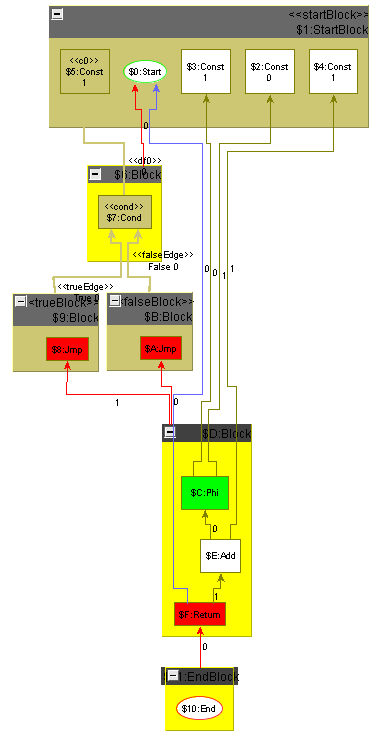
\includegraphics[width=2.89in]{fig/MinPlusCondMatched.png}
	}
	\qquad
	\subfloat[After folding the Cond.]{\label{fig:condfold}
		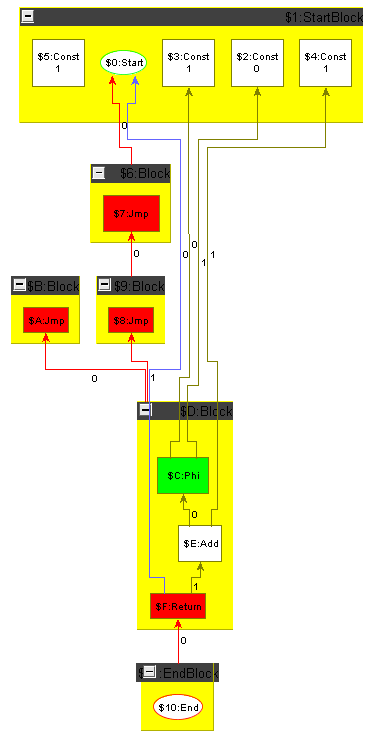
\includegraphics[width=2.7in]{fig/MinPlusCondRewritten.png}
	}
	\caption{Situation reached during folding the program graph of the minimum plus one function when applied to constant arguments.}
	\label{fig:cmpcondfold}
\end{figure}


%%%%%%%%%%%%%%%%%%%%%%%%%%%%%%%%%%%%%%%%%%%%%%%%%%%%%%%%%%%%%%%%%%%%%%%%%%%%%%%%%%%%%%%%%%%%%%%%
\section{Why to use \GrG}

\GrG\ offers processing of \emph{graph representations} at their \emph{natural level of abstraction}.

It is built on a \emph{rich and efficient metamodel} implementing multi-graphs, with multiple inheritance on node and edge types.
The nodes and edges are wired in scalable ringlists, which give access to their incident elements in constant time, to all elements of a type in constant time, and allow to add and delete elements in constant time.

\GrG\ features \emph{modular rules} that don't smear functionality into traversal code as is the case in traditional pointer structure passes.
It offers declarative \emph{graph patterns} of high expressiveness, saving you a lot of boilerplate code that would be needed for coding them manually.
And it implements efficient graph change rollback, thus allowing you to easily crawl search spaces without own bookkeping (for undoing the changes).

\GrG\ contains a C\#-like programming language, so you dont run against walls in case of subtask where the rules and patterns don't work well.
The \emph{general-purpose} system is highly extensible and customizable, you can express solutions fitting well to your task at hand.

\GrG\ offers the convenience of \emph{dedicated languages} with well-readable syntax and static type checking, instead of clunky internal DSLs, limited annotations, or annoying XML.
\GrG\ is brought to live by an \emph{optimizing compiler} that prunes not needed generality and generates pattern matchers adapted to the characteristics of the host graph at hand.
A runtime library is supplied that implements an easy-to-use API, and features built-in serialization / deserialization.

The system ships with a readily available shell application for file mapping tasks, which especially offers step-wise and \emph{visual debugging}, saving you from chasing reference chains in the debugger of your programming language.
Further mature development support is offered with search plan explanation and profiling instrumentation. 
Moreover, \GrG\ is properly documented in an extensive \emph{user manual}.

Traditional programming of graph representation processing is tedious, it requires careful orchestration of functionality attached to passes, boilerplate code for patterns, and low-level pointer fiddling.
You are more \emph{productive} with \GrG\ in coding a solution, but esp. are you so when changes are needed afterwards, a \GrG-specification can be adapted at a much higher pace.

Altogether, \GrG\ offers the \emph{highest combined speed of development and execution} for graph representation processing you can find.


